\begin{figure}[ht]
\centering
%\subfloat[First.]{...}%\qquad
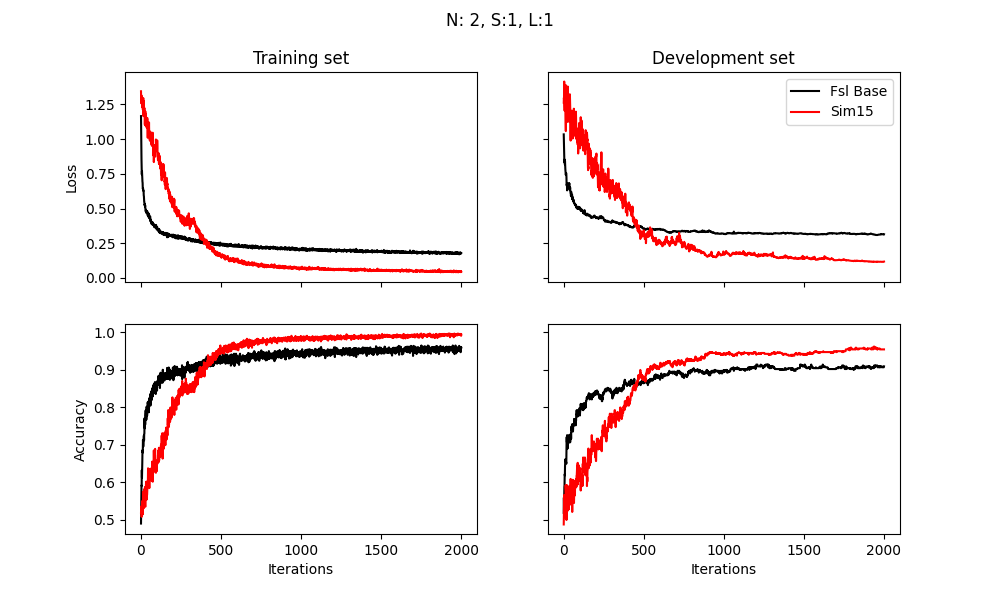
\includegraphics[width=0.49\textwidth]{figures/comparison/Epochs_2000--A_0.05--N_2--S_1--L_1.png}
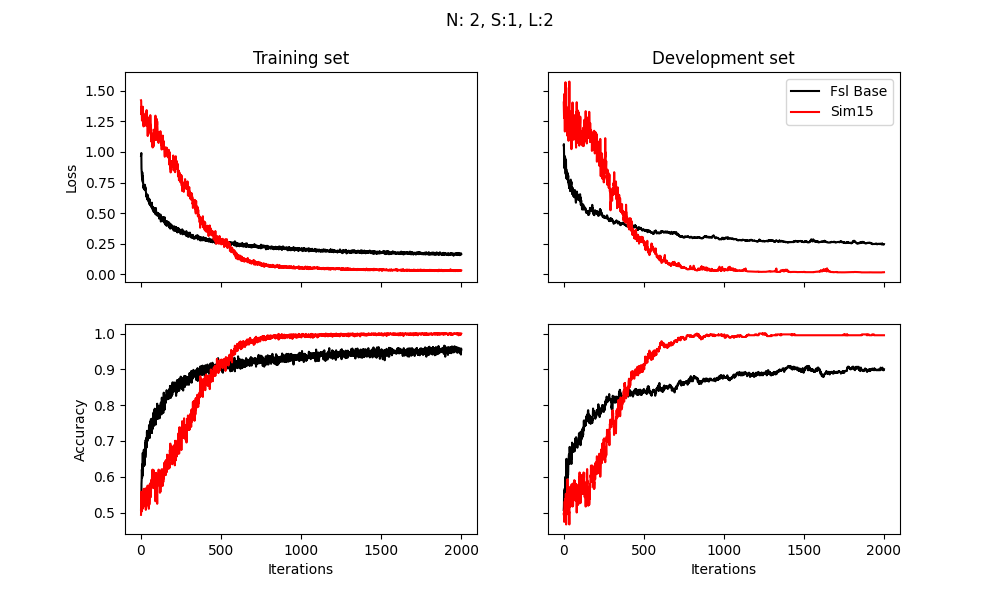
\includegraphics[width=0.49\textwidth]{figures/comparison/Epochs_2000--A_0.05--N_2--S_1--L_2.png}
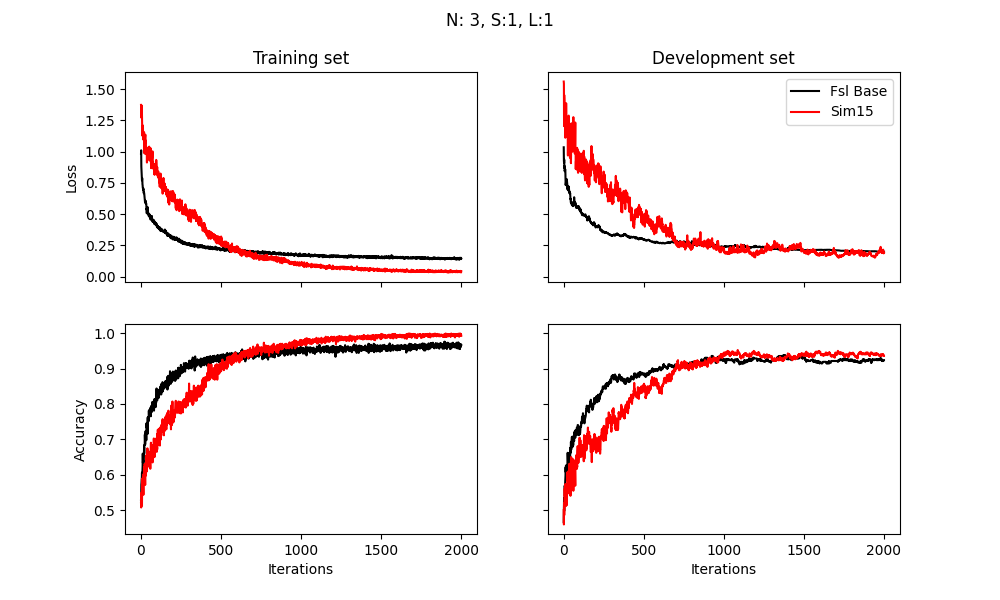
\includegraphics[width=0.49\textwidth]{figures/comparison/Epochs_2000--A_0.05--N_3--S_1--L_1.png}
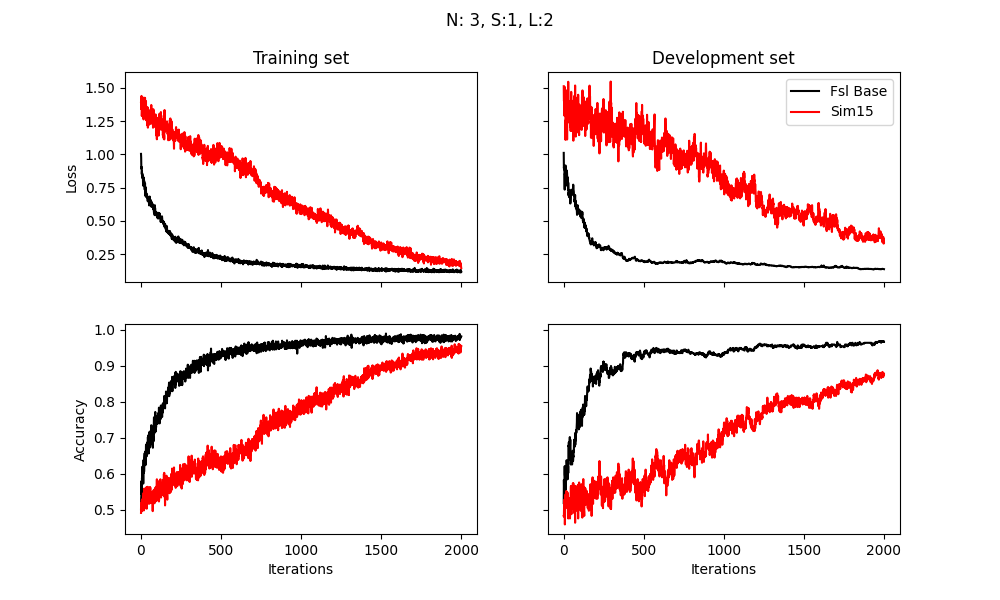
\includegraphics[width=0.49\textwidth]{figures/comparison/Epochs_2000--A_0.05--N_3--S_1--L_2.png}
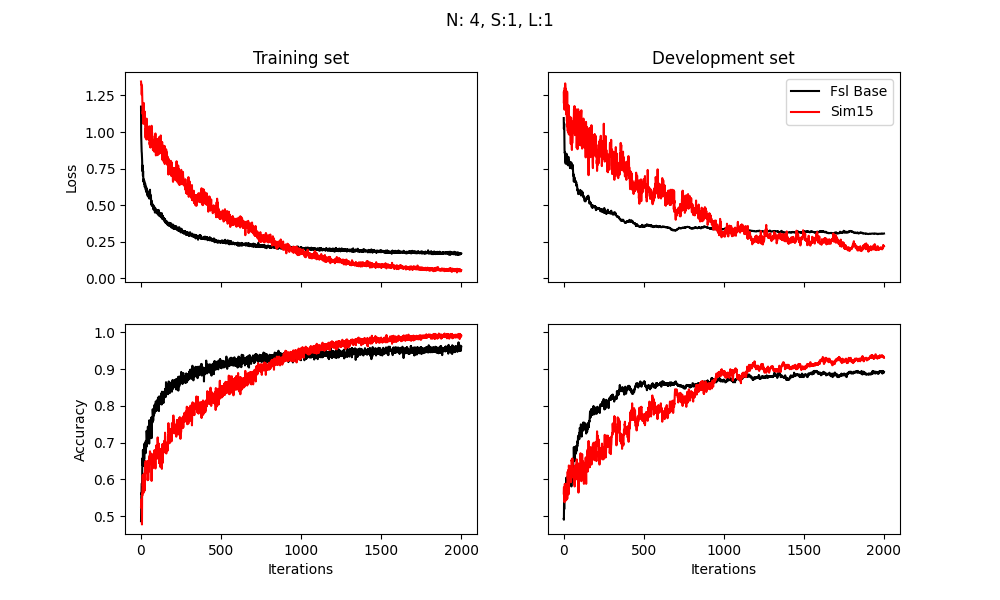
\includegraphics[width=0.49\textwidth]{figures/comparison/Epochs_2000--A_0.05--N_4--S_1--L_1.png}
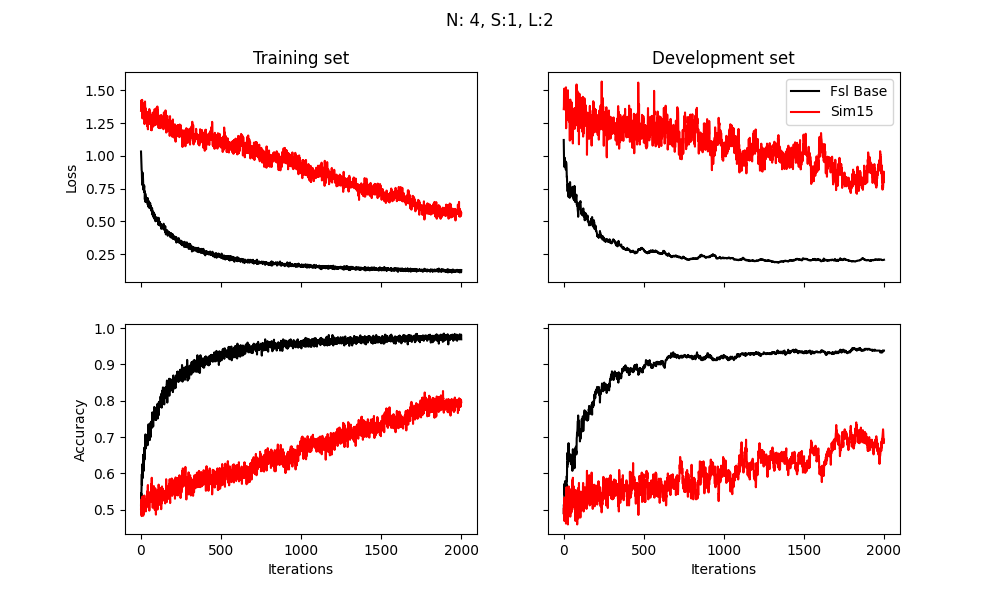
\includegraphics[width=0.49\textwidth]{figures/comparison/Epochs_2000--A_0.05--N_4--S_1--L_2.png}
\raggedright
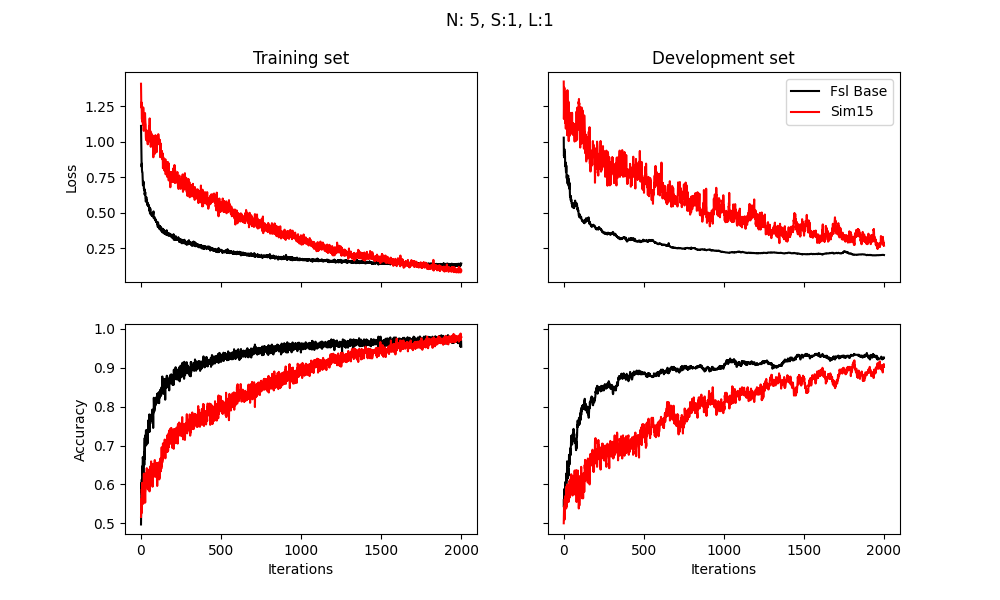
\includegraphics[width=0.49\textwidth]{figures/comparison/Epochs_2000--A_0.05--N_5--S_1--L_1.png}
\caption[Ans{\"a}tze behaviour comparison for small datasets]{Training behaviour for two types of \mya on the MC task after 2000 training Epochs.}
\label{fig:test1}
\end{figure}
